\subsection{Super Mario World}

We are going to focus on a single game for level generation:
\emph{Super Mario World}~(SMW). Super Mario World was released in~1990
by Nintendo for the Super Nintendo Entertainment
System~\cite{SuperMarioWorld2019}. It is a 2-dimensional platforming
game with the goal of reaching each level's exit in a limited amount
of time. Games in the platforming genre confront the player with
dangers like pits and enemies which have to be avoided by carefully
jumping and maneuvering across them in a host of levels. The original
game features 75~levels with 96~different exits (each level may have
more than one goal, especially secret goals). \\
The player has access to a moveset including but not limited to
running, jumping, picking up and throwing objects, and even shooting
fireballs, flying and riding a dinosaur extending the amount of
abilities even further. To access some abilities, Mario has to pick up
power-ups usually contained in ``question mark blocks''
(``?~blocks''). Blocks are commonly activated by hitting them from
below. During a level, the player may collect various items like the
power-ups mentioned above (which also let Mario take one extra hit
before he is defeated) as well as coins and one-up mushrooms which
increase the amount of lives (tries) available to the player. \\
Usually, when Mario lands on top of an enemy, the enemy is defeated.
There are some enemies which Mario cannot safely land on or cannot
defeat by jumping on top of them. Those enemies require a different
trick like throwing something at them or hitting a block they are
standing on from below. \\
Sometimes, the player may even have to use an enemy to complete a
level. For example, the turtle-like ``Koopas'' get knocked out of
their shell before being defeated. The shell has a variety of uses
like activating an unreachable block, defeating enemies and even
giving access to mid-air jumps by throwing and subsequently landing on
the shell.

The next two sections will give an in-depth look into why Super Mario
World was chosen as a machine learning problem and just how complex
the levels are. We will then give a more low-level overview into how
the levels work and what one has to look out for when creating a
database suitable for feeding into a machine learning model.

\subsubsection{Hacking Scene}
\label{sec:hacks}

At the time of writing, Super Mario World is almost 30~years old. Due
to both its age and success, it has been able to gain a large
following of people not only interested in playing the game but also
extending it. As with many other~-- especially retro~-- games, there is
a read-only memory (ROM) hacking scene around Super Mario World. In
this thesis, ``ROM'' will refer to the digital form of the Super Mario
World ROM cartridge that would usually be inserted into the Super
Nintendo Entertainment System; like the data that is burned onto a CD.
A lot of tools have been created to manipulate Super Mario World; even
in ways that the original creators hadn't programmed. People are able
to create their own levels and share them with the masses by uploading
a patch file that has to be applied to the original game
ROM\footnote{Usually the American version; CRC32 checksum
  \texttt{a31bead4}.}, thereby avoiding copyright infringement as
sharing the ROM, Nintendo's protected property, is illegal. The
program we use for applying patches is \emph{Floating
  IPS}~\cite{alcaroAlcaroFlips2019,FloatingIPSFlips}, or \emph{Flips}.

Due to the refined tooling available, users do not need to program in
65C816 assembly\footnote{The Super Nintendo Entertainment System's
  16~bit microprocessor is based on the 65C816 microprocessor.} to
modify the game. Instead, even non-technical users are able to use one
of the oldest tools to modify Super Mario World: \emph{Lunar
  Magic}~\cite{FuSoYaNicheLunar}. It features a GUI (that also enabled
some great visualizations) and has optional features that extend Super
Mario World with new functionality such as larger levels, custom coded
tiles, and more. The creator of Lunar Magic, \emph{FuSoYa}, modified
the existing software to support both dumping and reconstructing
levels, making this work possible due to the reduced workload of
parsing the data from the binary ROM. The features are currently only
available in a private build (based on Lunar Magic version~3.04) that
will be used throughout the thesis to (1)~parse level data from
existing ROMs and to (2)~write newly generated levels back into the
original Super Mario World ROM.

With Lunar Magic as a user friendly tool granting creators all the
freedom they could ever desire to design their own Mario levels,
communities around ROM hacking emerged. One of those communities is
\emph{SMW Central}~\cite{SMWCentralYour}, hosting most of the
available Super Mario World ROM hacks. Due to both SMW Central's
filtering capabilities and its quality of content, it was the source
for all levels used in this thesis (excluding the ones in the original
ROM). All the hacks used were obtained from SMW Central where their
respective authors (who are not necessarily related to SMW Central)
uploaded them.

Being able to filter hacks was important for two reasons. One being
that programmed custom behavior was out of the scope of this work,
requiring both parsing the binary 65C816 assembly code and then
understanding its every behavior. So we used the ``vanilla'' tag to
exclude hacks using behavior not in the original game (also called
the ``vanilla'' game; we will use these terms interchangeably). 
Also, to assert some form of quality in the dataset, only hacks with a
rating greater than or equal to~3.0 were downloaded (our rating is the
mean of all individual ratings, ranging from~1.0 to~5.0 and including
\emph{None} for no individual ratings). Sadly, some hacks are
protected via an encryption (possibly offered by Lunar Magic) and do
not allow reading their data; we had to omit all of these. All in all,
over 17\,000~unique levels in over 300~hacks were obtained thanks to
the community keeping a masterpiece alive and fresh for not only all
the years since the game's release but also for many years to come.
While this amount of data is not a lot relative to what deep learning
models usually train on in~2019 (with data points in the millions,
even approaching billions), it may be enough for our models to get a
grasp on what makes a level enjoyable.

Sadly, the ``vanilla'' tag is user-assigned, meaning users may label
hacks with some non-vanilla behavior as ``vanilla'' while others may
forget to assign the label at all, leaving us with both unclean and
less data than we would hope for. We include scripts to check for some
non-vanilla behavior and remove levels implementing those from our
dataset. A list of removed patches, ROMs and levels can be found in
the \texttt{stats} directory in the source code repository. \\
Finally, as mentioned, hacks operate on the real ROM as patches. Most
of the levels of the original ROM are usually untouched and remain the
same even after applying the patch. As we dump all levels contained in
a ROM, we remove these duplicated levels afterwards. If any one of the
dumped files is changed, we do not remove the level as it may be a
bonus level or a level solely containing the goal post (often used for
ghost houses). \\
In the original ROM, there are several duplicated ``test'' levels
which are also removed. Hack authors may also leave unfinished levels
or test levels in the ROMs which we cannot reliably detect. This will
``pollute'' our dataset a little but will hopefully not have a great
effect during training.

\subsubsection{Levels}
\label{sec:levels}

We already assessed that Super Mario World is a complex game with many
possibilities both in play and creative freedom in level design due to
the vast number of interactions in the virtual world. We will now fill
in some missing gaps of what makes up a level.

\begin{figure}[t]
  \centering
  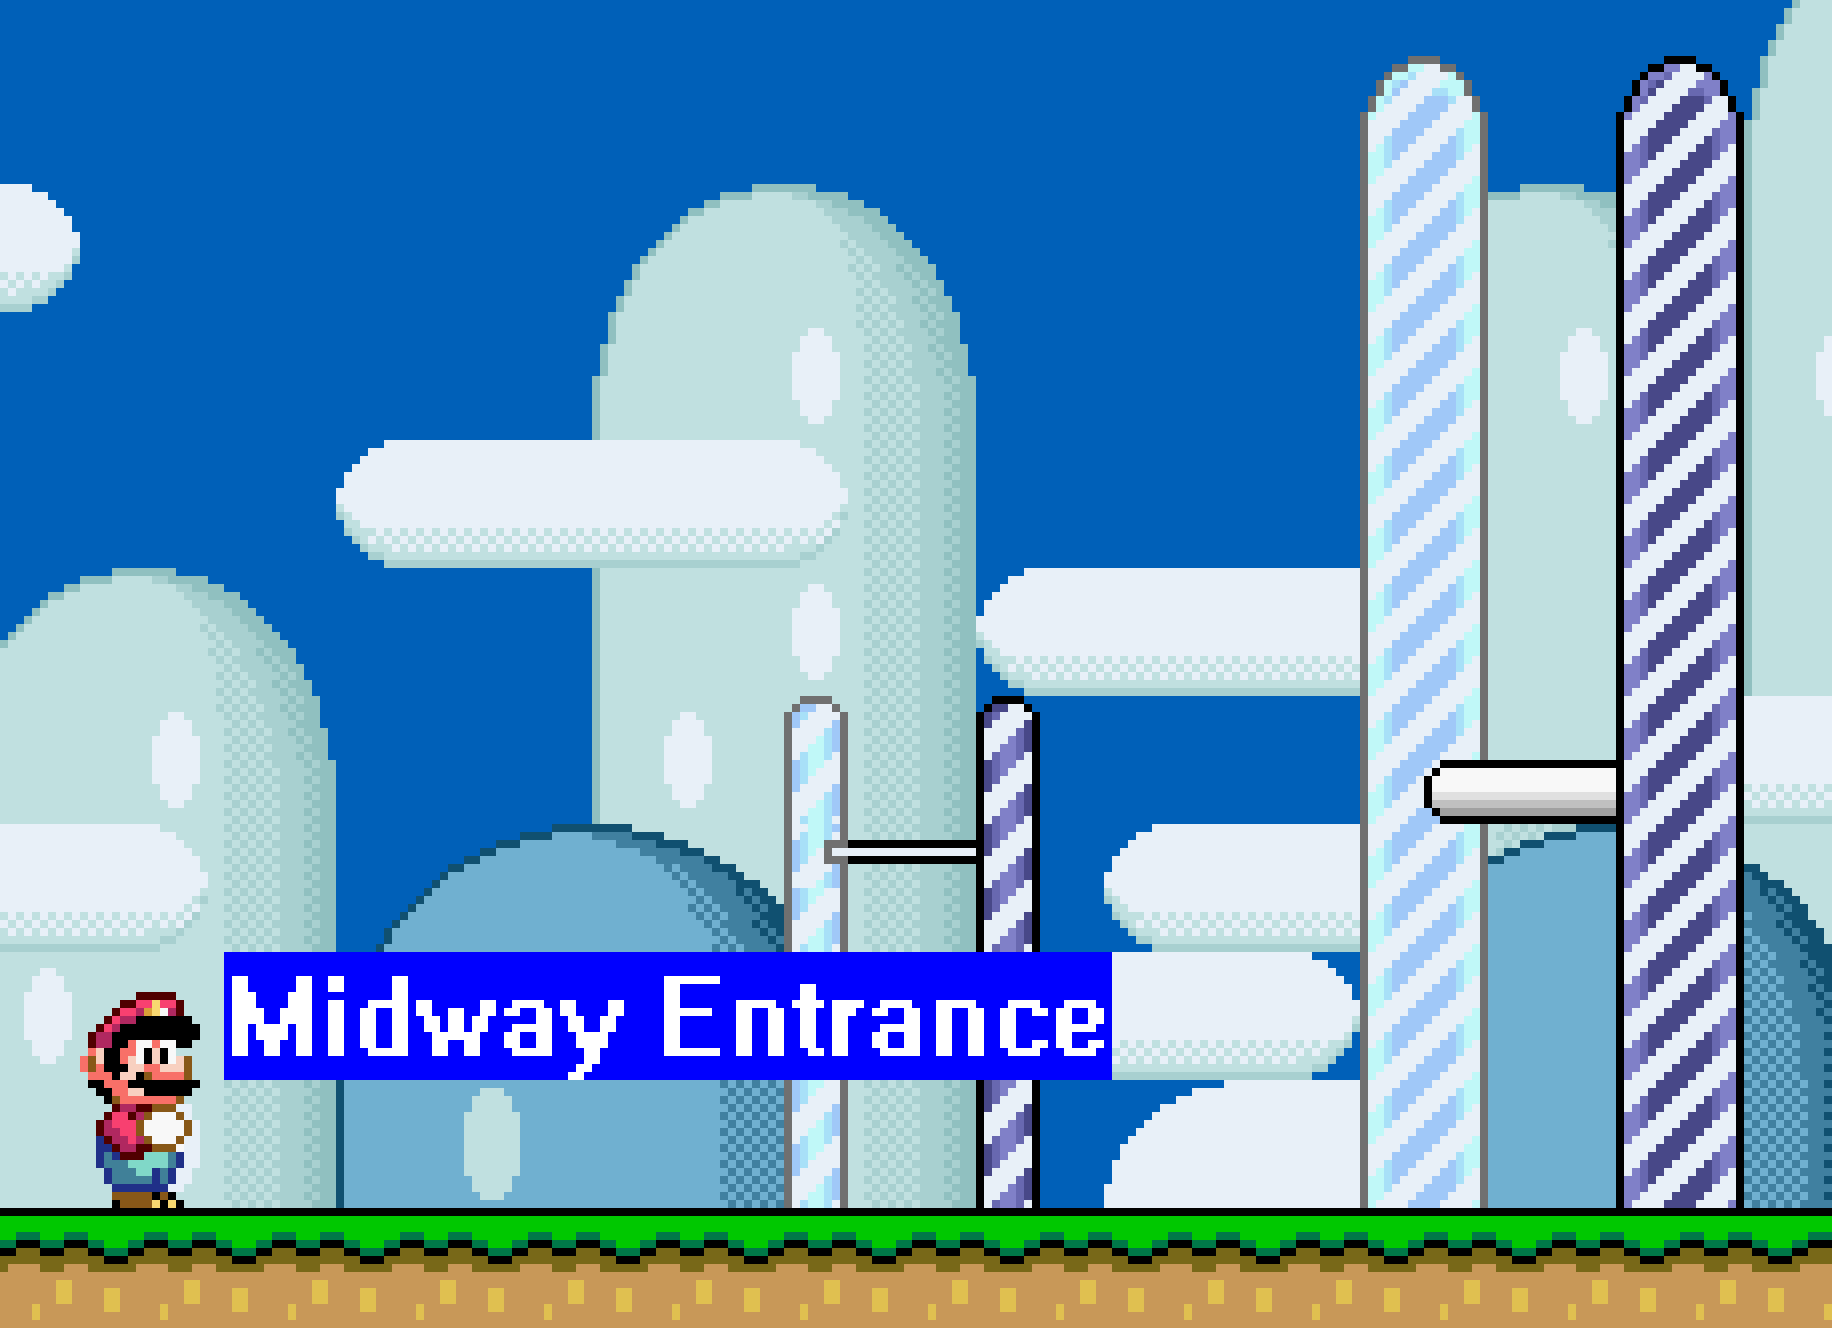
\includegraphics[width=\textwidth]{Level105_midway_goal.png}
  \caption{Aside from the midway and goal point, this figure also
    shows that the midway entrance is separate from the midway point.
    While the midway point consists purely of tiles, the moving goal
    point tape is actually a sprite.}
  \label{fig:midway-goal}
\end{figure}

To give the player an easier or less frustrating time, most levels
contain a \emph{midway point} (shown in figure~\ref{fig:midway-goal}).
When activated (achieved by touching the midway point tape), Mario
will spawn at that point instead of the usual level entry point in
case he is defeated. Most levels end when Mario reaches the goal post
(pictured in figure~\ref{fig:midway-goal}; touching the tape is not
required). Some levels end when Mario touches an orb while others end
when a key is transported to and inserted into a keyhole. Finally,
there are boss levels that are completed by defeating a boss. We will,
however, not consider these.

Each level may be connected to a number of other levels. The game
achieves this through two systems which will be explained in the
paragraph on layers on page~\pageref{par:layers}. The high-level
connection between two levels is given by tiles with special behavior
that can be entered by Mario. These tiles are called ``exit-enabled''
tiles. The most common are doors and pipes (only some pipes are
exit-enabled; those cannot be visually distinguished from those which
aren't).

Levels can have underwater regions through which Mario will have to
swim, removing his ability to jump on enemies to defeat them. Some
levels are vertical, growing in height rather than width. Other levels
are covered in darkness, where light is only emitted in a small radius
around Mario while others automatically scroll the level forward,
forcing the player to react more quickly and not get stuck on a wall
(when the level scrolls beyond Mario, he is defeated). Finally, a
level may contain ``blue P~switches'' that temporarily turn coins into
blocks and certain blocks into coins, granting new paths to the player
that are possibly required to reach the goal. A very similar tile is
the ``gray P~switch'' which spawns coins and special doors.

All these different tiles can be combined in any way imaginable. Most
of those combinations in the high-dimensional level space are
non-playable nonsense. However, as described in
section~\ref{sec:hacks}, due to the large amount of possible~-- and,
more importantly, enjoyable~-- interactions between all the different
pieces contained in the original game, a seemingly infinite number of
unique, fun levels can be created.
\medskip

We are now going to leave the high-level view of levels and take a
look at how everything works together on a lower level: \\
Levels are made up of \emph{screens}; matrices of the same size. Each
screen is made up of two subscreens; in horizontal levels, subscreens
are stacked vertically and the whole, combined screens are
concatenated horizontally while in vertical levels, subscreen are
stacked horizontally and screens concatenated vertically. While
subscreens are important in data preparation, we will not focus on
them in this work and instead always refer only to whole screens. A
screen is a 2-dimensional slice of the level consisting of a number of
columns and rows. Screens in horizontal and vertical levels have
different sizes (even if horizontal screens are transposed), but
otherwise, screen sizes are constant over different levels. While
Lunar Magic supports non-vanilla behavior in that screens can have
other sizes (although still a constant size per level). Like with all
non-vanilla modifications that have a direct impact on data, we are
going to ignore that feature. For simplicity, we are also only going
to train on horizontal levels. While support for vertical levels in
database generation exists, models that support both types of levels
are more complicated. Also, vertical levels only make up a fraction of
total levels, so not a lot of data is lost (circa~2\,000 of the over
17\,000~levels are vertical).

Calling a screen a matrix is not the whole truth. While screens itself
are basically only areas in a level, those areas can contain many
different layers of other types of objects.

\begin{figure}[t]
  \centering
  \makebox[\textwidth]{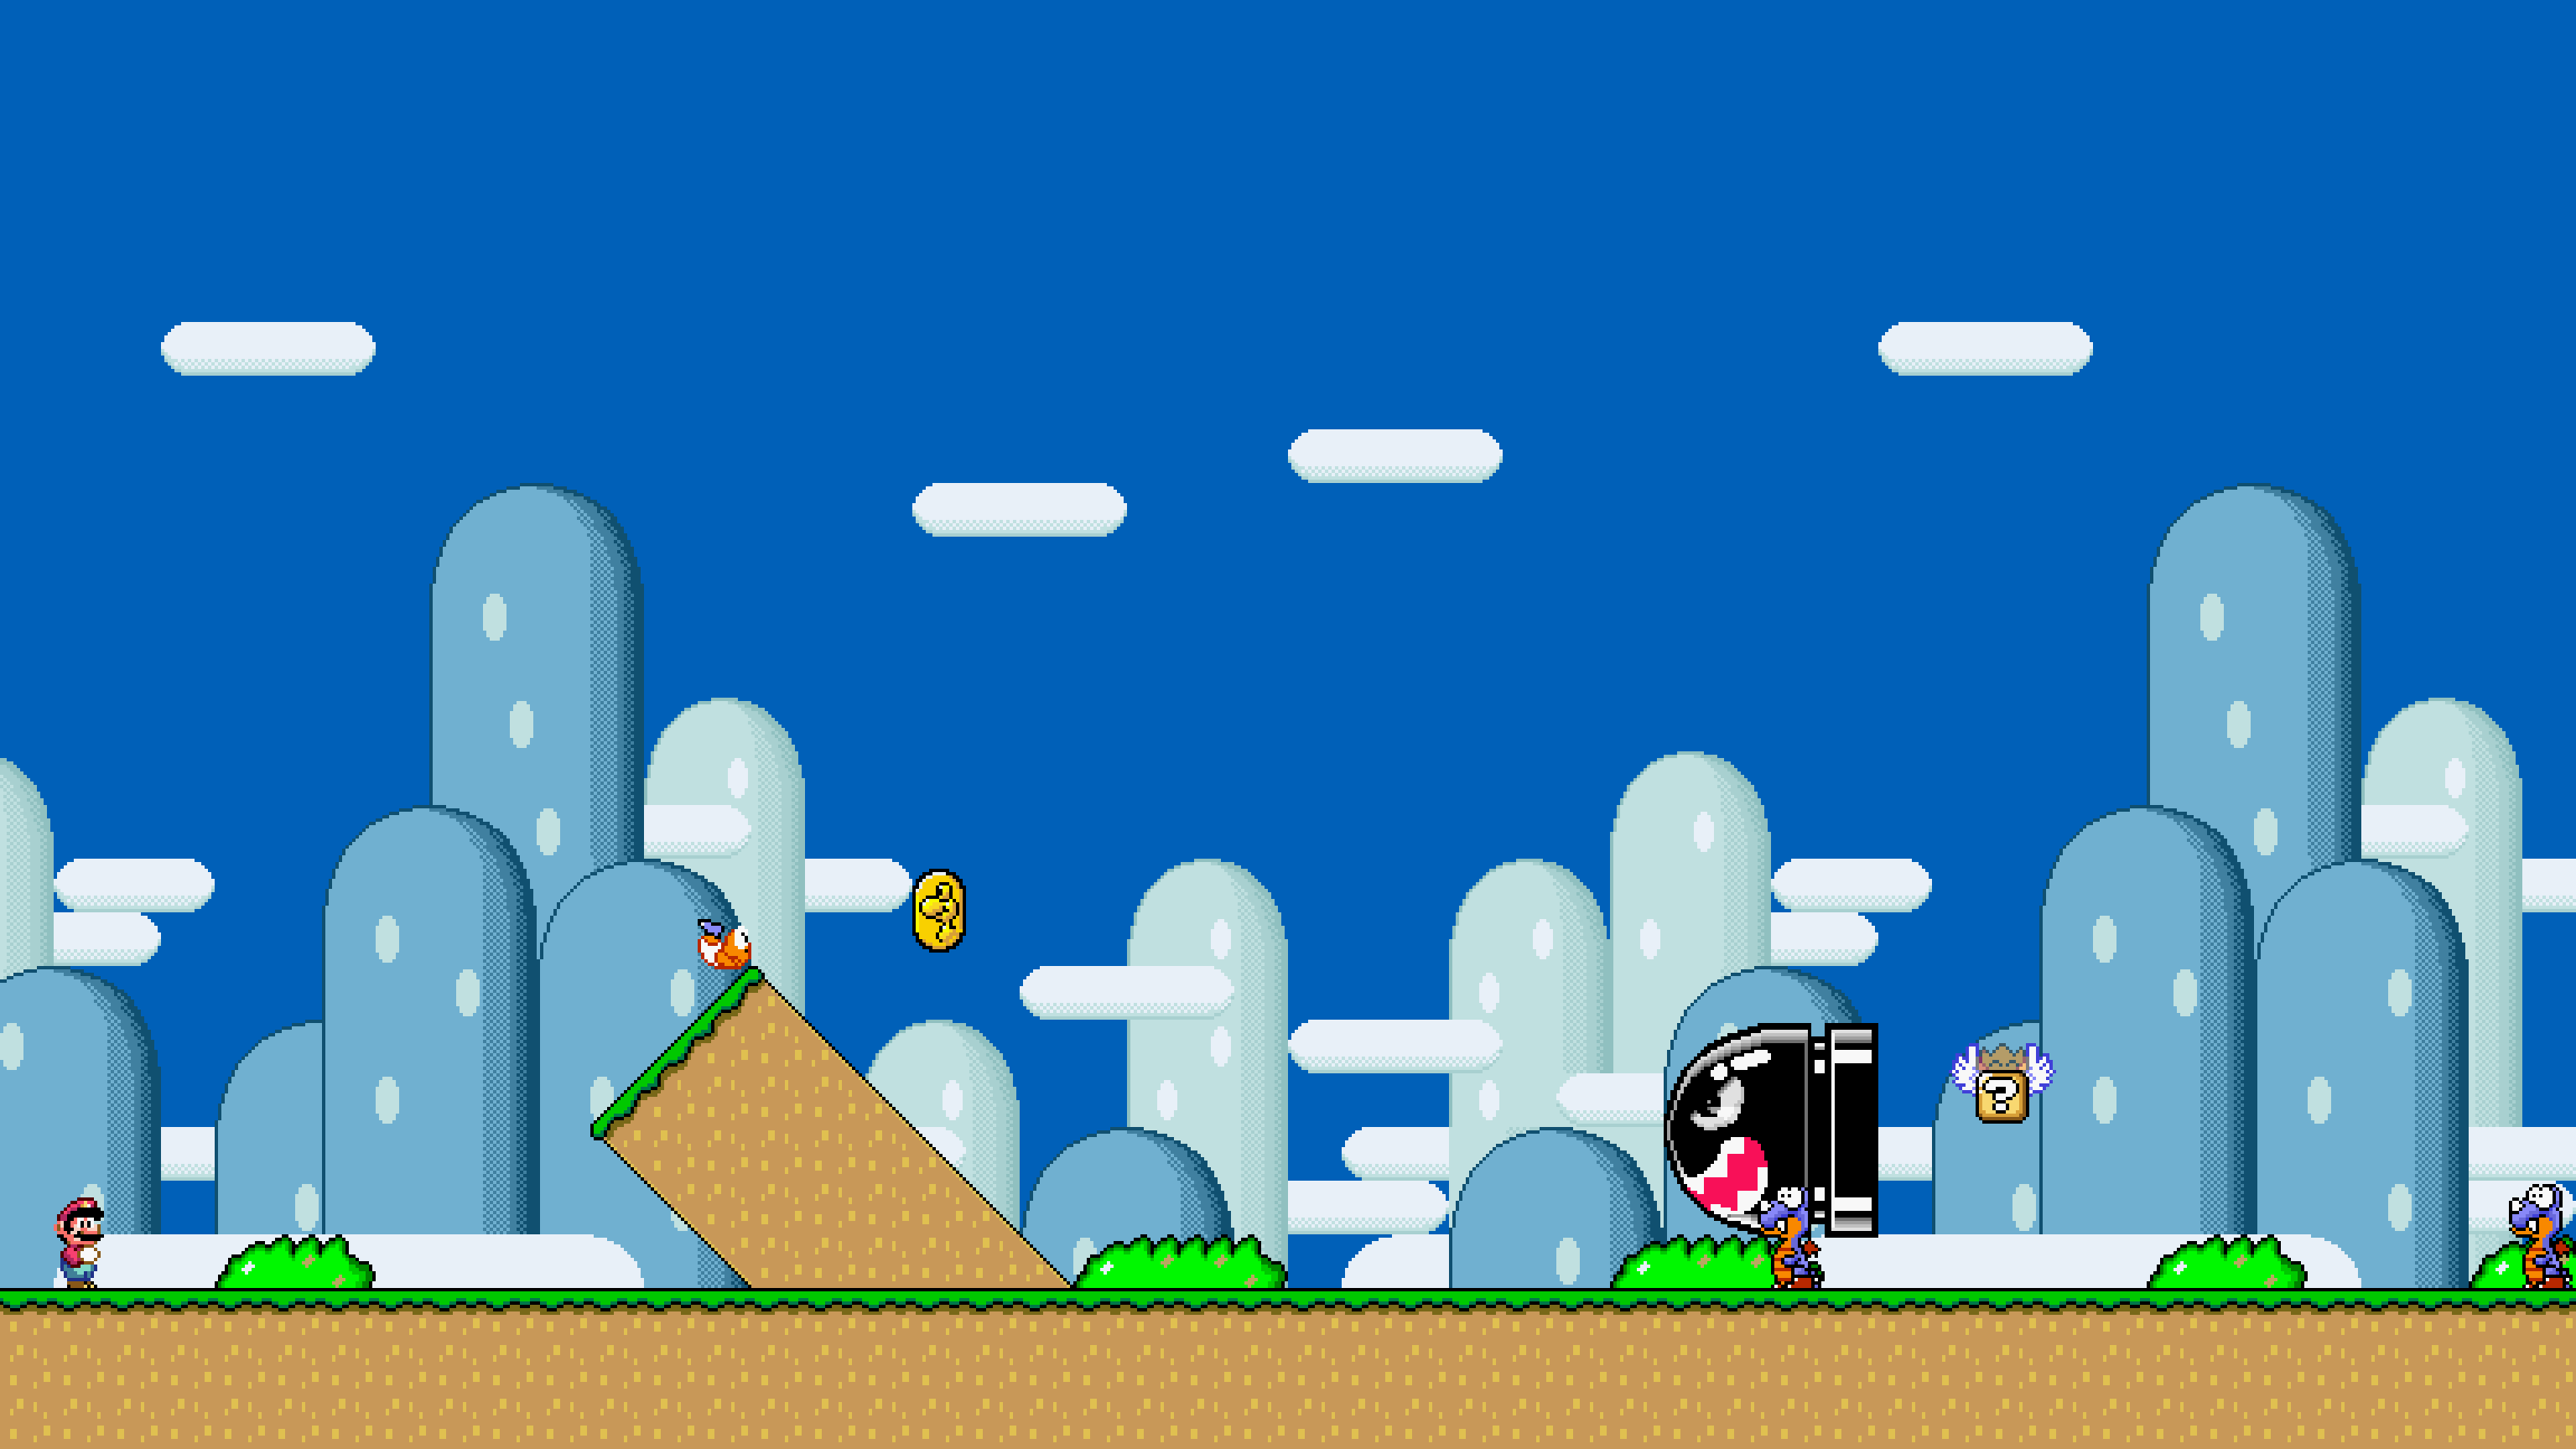
\includegraphics[width=1.2\textwidth]{Level105_clean.png}}%
  \caption{The first three screens of level~261. The main entrance
    point is depicted as Mario.}
  \label{fig:105-clean}
\end{figure}

\begin{figure}[t]
  \centering
  \makebox[\textwidth]{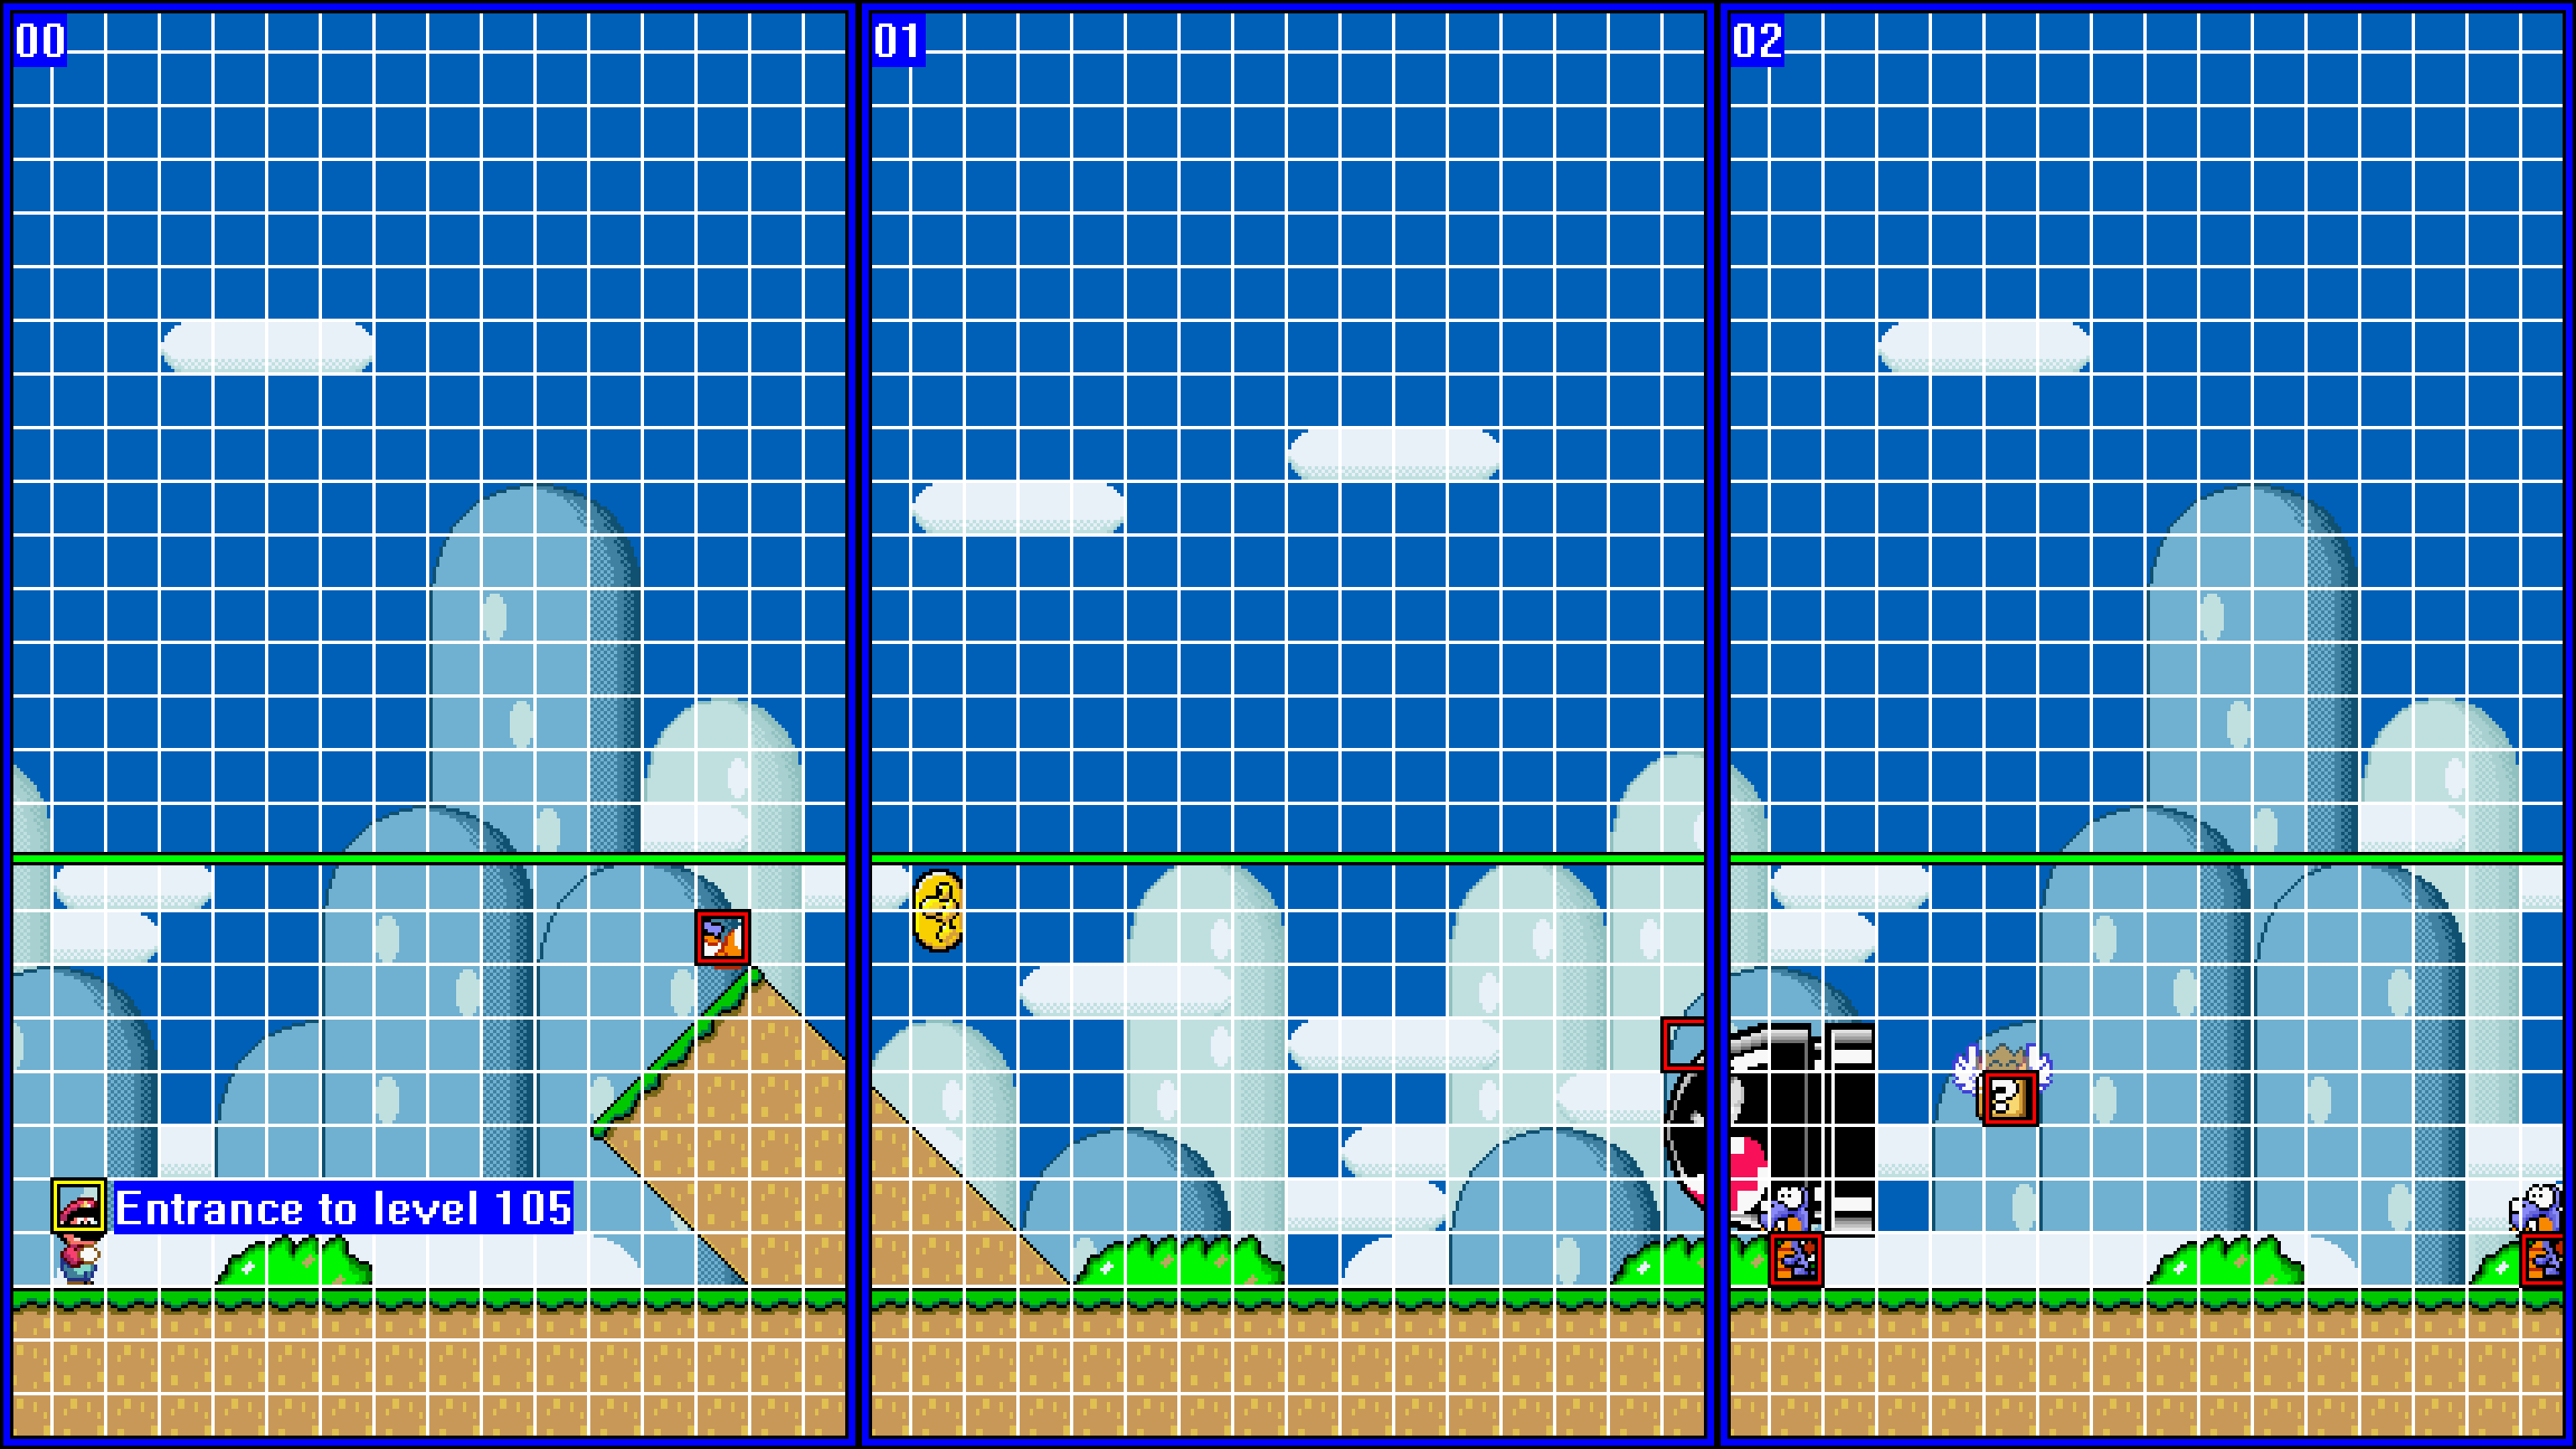
\includegraphics[width=1.2\textwidth]{Level105_detailed.png}}%
  \caption{The first three screens of level~261 with detailed
    information and a white grid distinguishing individual tiles.
    Screens edges are blue with their hexadecimal number at the top
    left; the green line in the middle indicates subscreen boundaries.
    The position of the main entrance has a yellow border. The actual
    positions of sprites containing information have a red border.}
  \label{fig:105-detailed}
\end{figure}

\paragraph{Layers}
\phantomsection
\label{par:layers}

While we will explain ``layers'' in this section, in the hacking
community, the term ``layer'' refers to both interactive and graphical
tilemaps (of which there are three of). When we refer to the second
meaning, we will explicitly list a number behind the layer (for
example ``layer~2''). \\
Aside from the previously explained screens, levels consist mainly of
five different \emph{object types} which each correspond to a file
dumped by Lunar Magic. Also, each of these object types needs many
layers that contain all the data. The types and a short description
are listed here:
\begin{enumerate}
\item \emph{Tiles} are most of the static blocks in a level. They
  usually make up the ground, platforms, walls and ceiling of a level
  (if present). Also, most collectibles that are immediately visible
  in the level are a tile; examples are coins or moons\footnote{Moons
    give the player three lives upon collection.}. Some special tiles
  like doors and some pipe tiles are exit-enabled, meaning they lead
  out of a level (exits are described below). Even non-interactive
  background objects like arrow signs or bushes that only exist for
  aesthetical reasons are tiles. In the hacking community, this layer
  of tiles is also called ``layer~1''. \\
  The original game supports 512~tiles, each with possibly different
  behavior. Lunar Magic extends the amount of tiles by allowing users
  to define new, custom tiles that either (1)~reference another tile's
  behavior (these references may recurse but not loop), so only
  changing the texture of the tile or (2)~point to a custom procedure,
  so possibly changing both, the texture and the behavior of the
  tile. Due to only allowing vanilla hacks that promise not to
  implement custom behavior, we can ignore the second case and simply
  follow references until finding one of the original tiles. \\
  As mentioned at the beginning of this paragraph, tiles may exist on
  two layers in the level. Layer~2 may contain interactive objects or
  just non-interactive graphical background data. A special property
  of layer~2 tiles is that they can move if desired (how that is
  achieved will be described in a bit). When layer~2 is used for
  interactive tiles, it cannot act as a background tilemap. Therefore,
  a third (strictly non-interactive) layer exists for the sole purpose
  of a background tilemap which is usually in layer~2. This layer~3 is
  not related to tiles in any way. For simplicity, we ignore all data
  in layers~2 and~3.
\item \emph{Metadata} is any data that changes the behavior of a
  level without belonging to a certain position in the level. For
  example, which tileset (that is, the graphics) or which background
  music is used in a level is decided by the metadata. A level's
  metadata also contains its entry points. Finally, metadata may even
  change the behavior of certain tiles. We will describe metadata in
  detail in its paragraph on page~\pageref{par:metadata}.
\item \emph{Entrance points} are the positions of the main and midway
  entrances.
\item \emph{Sprites} are usually moving or movable objects that
  interact with Mario and each other in a certain way. For example,
  enemies and even goal objects like the orb, key and keyhole
  (described in section~\ref{sec:levels}) are sprites (while the goal
  post is a tile, the moving tape Mario can cross through is also a
  sprite). \\
  Sprites may also have other effects on the level; for example,
  sprites control auto-scroll behavior in a level or the movement of
  layer~2 tiles. Sprites may also affect a level's lighting or
  background objects. When Mario reaches a screen with one of those
  special sprites, the behavior will activate.
\item \emph{Exits} connect one level to another. An exit is
  screen-based, meaning it will be used by all exit-enabled tiles in
  the screen the exit is contained in. There are two types of exits:
  \emph{Screen exits} send Mario to an \emph{entrance point}
  (described above) of another level while \emph{secondary exits} can
  send Mario to a designated point in the level to be entered,
  described below.
\item \emph{Secondary entrances} are the destinations of secondary
  exits. These destinations cannot lie anywhere; they have certain
  pre-determined positions based on a table of positional values and
  based on whether they are in the first or second subscreen of the
  screen the secondary entrance lies in. Any number of secondary exits
  may point to the same secondary entrance.
\end{enumerate}

\begin{figure}[p]
  \centering
  \makebox[\textwidth][c]{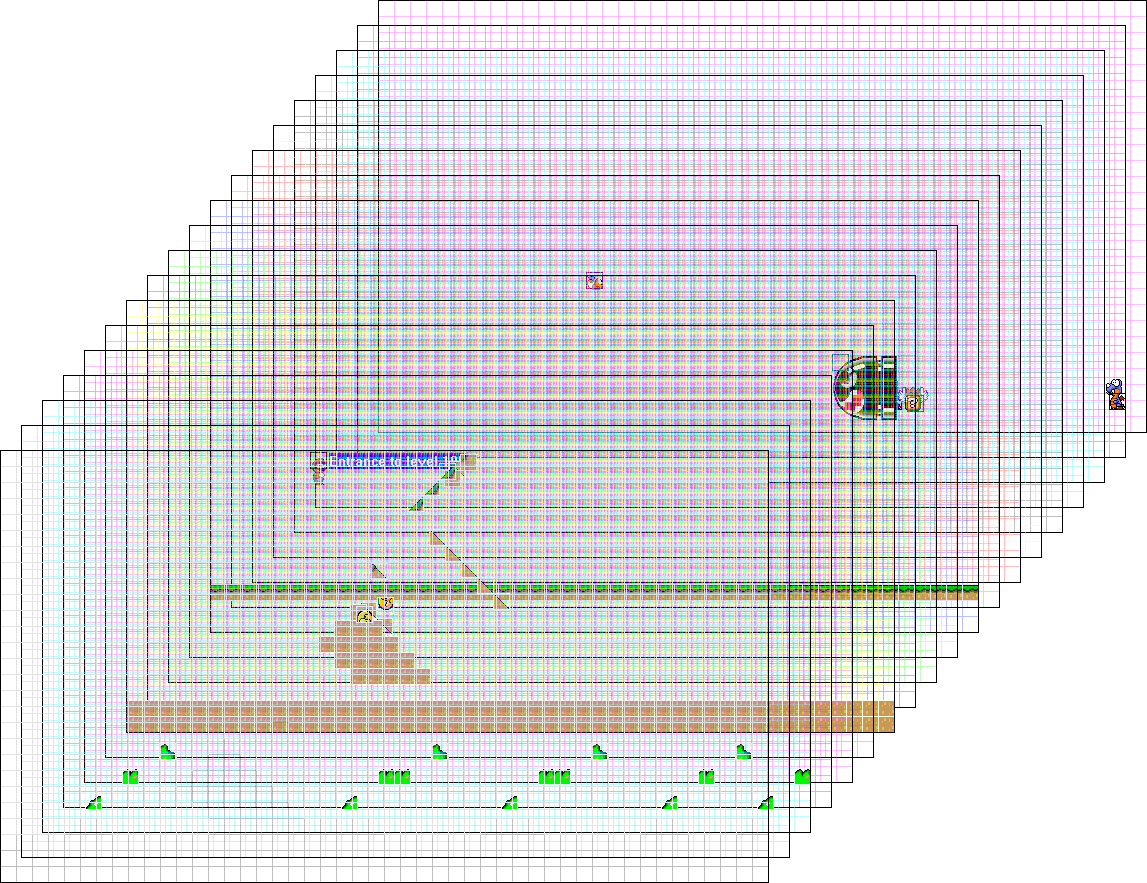
\includegraphics[width=1.5\textwidth]{Level105_layers_grid_border_grid_grouped_rainbow.png}}%
  \caption{The first three screens of level~261 shown as individually
    sliced layers in order of our abstract representation. The layers
    contain in order (an asterisk marks a non-interactive tile):
    (tiles)~empty tile*, bush left*, bush middle*, bush right*, Yoshi
    coin top, Yoshi coin bottom, ground background*, slope right
    corner, slope left edge*, slope right edge*, ground, slope top
    edge, slope top underside*, slope left corner, (entrance
    points)~main entrance, (sprites)~flying ?~block, Bullet Bill, Rex,
    sliding Koopa without shell. \\
    \medskip
    Each layer has a grid, where the colors cycle through black and
    rainbow colors for each layer. Tiles are highlighted with a
    brighter color. Elements in the grid other than tiles containing
    the actual position are highlighted in a darker color. Note that
    the converted data contains a lot of empty layers not visible
    here. \\
    \medskip
    In the abstract representation, each highlighted grid element
    becomes a~1; everything else is~0.}
  \label{fig:sliced}
\end{figure}

Now that we have described the different kinds of object types we will
be dealing with, we will take a quick look at how they expand in the
abstract space our model is going to work with. It should be noted
that each object type contains individual \emph{type instances} (for
example, each unique type of tile like ``ground ledge block'' or
``gray cement block'' is a type instance of the object type ``tile'').
Each of these type instances regards its own layer to get a binary
encoding of the level. Figure~\ref{fig:sliced} may be helpful to
understand what we mean. Prior to constructing our data, we need to
know the amount of layers. We already know that there are 512~unique
tiles in the vanilla game. For the sprites, we need the amount of
unique sprites used over all hacks. To represent all possible exits,
we need the maximum amount of screen exits and connected secondary
exits and secondary entrances. In each hack, we count the amount of
screen exits and connected secondary exits and secondary entrances and
take the maximum of each of these over all hacks. We also need
2~layers to represent the level's main and midway entrance points. If
we sum up the total amount of all unique tiles and sprites, the
maximum amount of screen exits and (connected) secondary exits and
secondary entrances plus the two entrance points, we get a total of
$512 + 241 + 511 + 449 + 449 + 2 = 2164$ layers. A horizontal level
consists of 27~rows and at maximum $16 \cdot 32 = 512$ columns (16~columns
per screen, 32~screens at maximum). We may therefore get a maximum
amount of $27 \cdot 512 \cdot 2164 \approx 30 \cdot 10^{6}$ entries in the abstract,
binary representation of a level. \\
As the dimensionality of levels containing all layers is quite high
(and mostly filled with emptiness), we provide filters to only process
chosen level data making training both easier and faster. We even
provide a filter so only sprites directly relevant to reaching the
goal are kept. Due to Super Mario World's complexity, we cannot cover
each case. Sometimes jumping on an enemy or throwing a Koopa's shell
may be required to finish the level. These are just some examples of
the vast majority of possibilities. The filter should include most~--
if not all~-- sprites required for reaching the goal in the vanilla
game, though. These filters will be described in detail in
section~\ref{sec:preprocessing}.

We will now take a look at the effects a level's metadata has on it.

\paragraph{Metadata}
\phantomsection
\label{par:metadata}

As already explained, metadata contains information about a level that
is not related to any position in the level like changing a level's
graphics or music. However, even these effects may influence unrelated
objects. For example changing a level's fore- and background graphics
automatically changes the behavior of some certain tiles. Some tiles
may only exits for certain graphics settings. Due to these interactive
influences metadata has on a level, we need to take it into account
when training our model. Each level has three headers containing
metadata. A primary and a secondary level header and a sprite header.
While we could feed our model all the different metadata points, we
are only interested in the ones that provide information on two
issues: (1)~changes to interactive parts of the level and (2)~changes
to a level's size or ``vanilla-ness''. We need~(1) so our model may
learn the correct representation of each tile for each level and we
need (2)~to be able to filter undesired levels. As an example for~(1),
we already mentioned the graphics setting and its influence on tiles.
An example for~(2) is how many screens the level contains or whether
the level uses Lunar Magic's expanded format or whether it's a
horizontal, vertical, or even boss level. \\
Finally, positional information about the main and midway entrance of
each level is also stored in the metadata. We, however, do not treat
these as metadata and instead store them in the level matrix like
tiles.

Let us now take a look at how Mario levels are different from levels
in other games; at what makes them special and how it influences our
decisions regarding model design.

\paragraph{Comparison with Levels in Other Games}

While Super Mario World levels mostly follow a linear style of getting
from one side of the level (the beginning) to the other (the goal),
some levels include non-linearities. Levels may even loop and require
the player to solve a puzzle in order to progress or backtrack after
acquiring an object. Or after activating a P~switch in one level, a
door in another may suddenly appear. These influences on both a
level's linearity and its interaction with other levels makes it hard
to get a general generative solution for a level. We therefore
restrict our problem to only generating one independent level each,
not a level including the levels its exits point to. This means that
we will get incomplete levels or unconnected exits. One way of
addressing this would be to generate a more holistic view, meaning
concatenating a level to its connected levels and generating all at
once. Even then, we would need to interpret the way the level plays
out to concatenate the levels in the right order. Due to the immense
increases in architectural (software) and model complexity, this is
reserved for future work.

In Super Mario World, each level is independent from another
(excluding levels connected by screen or secondary exits)\footnote{A
  counter example is Super Metroid~\cite{SuperMetroid2019}, also
  released on the Super Nintendo Entertainment System, in which the
  whole world is in concept one giant level, also divided into
  screens.}. This means we will not have to pay attention to Mario's
state in between different levels. For example, in other games, a
permanent power-up may be required to progress in a future level. We
do not have this issue, enabling us to start fresh with each level we
generate. In the same vein, as levels are not connected with each
other (again, excluding the connections by screen or secondary exits),
our problem size shrinks as we do not need to get a complete view of
the whole game world. While the original game separates levels into
different biomes or worlds (grassland, cave, forest, \dots) by
changing the graphics of sequential levels to the corresponding theme
(based on metadata), some hacks may tell a story by tuning the general
feel and environment of one level to fit the following one. We can
ignore this and still obtain a new, interesting Super Mario World
game, even though the cosmetic, meta-view of the world whose story is
told through the game, is lost.

With that, we have described the most important concepts in Super
Mario World and how they influence our decisions regarding model
design and data selection. We will now explain the machine
learning-related methods used throughout this work in detail.

%%% Local Variables:
%%% mode: latex
%%% TeX-master: "../../SMWLevelGenerator"
%%% End:

